\documentclass[12pt,american,UTF8]{article}
\usepackage[UTF8]{ctex}
\usepackage[T1]{fontenc}
\usepackage{fourier}
\usepackage[hidelinks]{hyperref}
\usepackage{babel}
\usepackage[babel]{microtype}
\usepackage[babel]{csquotes}
\usepackage[journal={IEEE Transactions on Neural Networks and Learning Systems},
			manuscript={TPAMI-2024-11-3068},
			editor={Mrs. Joyce Arnold}]{reviewresponse}
			
\usepackage{fancyhdr}
\usepackage{lastpage}
\usepackage[a4paper,total={160mm,245mm},left=25mm,top=25mm]{geometry}
\renewcommand{\headrulewidth}{0pt}
\renewcommand{\footrulewidth}{.5pt}
\usepackage[shortlabels]{enumitem}
\newlist{detail}{itemize}{3}
\setlist[detail, 1]{label=\textbullet,leftmargin=21pt,nosep}
\usepackage[backend=biber,style=ieee,dashed=false,url=false,isbn=false,defernumbers=false,refsection=section]{biblatex}

\usepackage{amsmath,amsfonts}
\usepackage{graphicx}
\usepackage[table]{xcolor}
\usepackage{multirow}
\usepackage{booktabs}
% \usepackage{colortbl}
\usepackage{pifont}
\usepackage{makecell}
\usepackage{threeparttable}
\usepackage{extarrows}
\usepackage{bm}
\usepackage{enumitem}
\setlist[enumerate]{itemsep=2pt, parsep=0pt, topsep=4pt}
\usepackage{enumitem}
\setlist[itemize]{itemsep=2pt, parsep=0pt, topsep=4pt}

\usepackage{multicol}
\usepackage{csquotes}
\usepackage{arydshln}

\usepackage{hyperref}
\usepackage{caption}

\usepackage{lipsum}
\usepackage{listings}
\usepackage{threeparttable}

\usepackage{xcolor}
\usepackage{colortbl}
\definecolor{color1}{rgb}{0.9764,0.8039,0.6784}
\definecolor{color2}{rgb}{0.7843,0.7843,0.6627}
\definecolor{color3}{rgb}{0.5137,0.6862,0.6078}

\newcommand{\dyfdraft}[1]{\textcolor{gray}{#1}}
\newcommand{\dyfcomment}[1]{\textcolor{red}{\bf [Comments: #1] }} 

\usepackage{amsthm}
\theoremstyle{plain}  %plain,definition,remark
\newtheorem{theorem}{Theorem}
\newtheorem{definition}{Definition}
\newtheorem{lemma}{Lemma}
\newtheorem{corollary}{Corollary}

\usepackage{algorithm}
\usepackage{algorithmic}

\usepackage{tikz}
\def\checkm{\tikz\draw[thick,scale=0.2] (0,0.4) -- (0.4,0) -- (1,1);}
\newcommand{\halfcheckm}{%
	
\begin{tikzpicture}[scale=0.2]
		\draw[thick] (0,0.4) -- (0.4,0) -- (1,1);
		\draw[thick] (0.5,1) -- (1,0.3);
	\end{tikzpicture}%
}
\newcommand{\fork}{%
	
\begin{tikzpicture}[scale=0.2]
		\draw[thick] (0,1) -- (1,0);
		\draw[thick] (0,0) -- (1,1);
	\end{tikzpicture}%
}

\hypersetup{
	colorlinks=true,
	linkcolor=blue,   % 设置链接为蓝色
	citecolor=blue,
	urlcolor=blue,
}


%\bibliography{literature.bib}
\addbibresource{literature.bib}

% \definecolor{lightblue}{RGB}{60, 39, 139}

\title{Accurate and Efficient Binarized Transformer by Algorithm-Hardware Co-design}

% If you do not need author information (double-blind review), please modify the \renewcommand*{\maketitle} function in reviewresponse.sty
\author{FirstAuthors (Institution1; FirstAuthors@126.com)\\
		SecondAuthors (Institution2; SecondAuthors@126.com)}


\begin{document}
\maketitle

\tableofcontents

% Cover Letter
%\clearpage
\thispagestyle{empty}
\clearpage
\phantomsection
\addcontentsline{toc}{section}{\protect\numberline{}Cover Letter}

\noindent \textbf{Dear Editors, Associate Editor and Reviewers:}

Thank you for your valuable and insightful feedback on our manuscript, ``Accurate and Efficient Binarized Transformer by Algorithm-Hardware Co-design''. We greatly appreciate your time spent reviewing our manuscript and making constructive suggestions, which have greatly improved the quality of our manuscript. In light of the reviewers' comments and recommendations, we have meticulously revised the manuscript and provided a detailed point-by-point response. Furthermore, we have meticulously reviewed and corrected the manuscript to ensure no errors. We hope that our revisions and responses will meet with your satisfaction.


\paragraph{What We Added in the Revision}

\begin{itemize}
    \item \textbf{Broader baselines}: Integrated the works listed above into the Related Work and, where possible, the experimental comparisons.
    
    \item \textbf{Extend to LLMs}: Implemented our method on representative LLMs, covering both training algorithm and custom CUDA kernels, and evaluated on WikiText-2, C4, CommensenseQA benchmarks under standard LLM protocols.

    \item \textbf{Training dynamics}: Report LLM training loss curves to demonstrate the transferability and stability of our method beyond the BERT setting.

    \item \textbf{Reported end-to-end latency, operator-level throughput, and GPU memory footprint} in both prefill and decode phases with various batch sizes and sequence lengths to make the system-level gains explicit. 
    % End-to-end speedup and operator-level throughput: Provide end-to-end timing comparisons on both prefill/decode phases, and operator-level timing against linear acceleration implementations to make the system-level gains explicit.

    \item Revised narrative: Concise, shortening and focused presentation. 
\end{itemize}


We want to take this opportunity to thank you for handling our manuscript, and we look forward to hearing from you.

\vspace{8em}

\noindent Sincerely,

\noindent Authors

\vfill
\textbf{Note:} To enhance the legibility of this response letter, all the editor's and reviewers' comments are typeset in boxes. \textbf{In the revised manuscript, modified parts are marked in red, and newly added parts are marked in blue.}
\setcounter{page}{0}
\pagestyle{fancy}
\fancyfoot[R]{\thepage\ / \pageref{LastPage}}
\fancyfoot[L]{Response Letter for TPAMI-2024-11-3068}
\fancyfoot[C]{\ }


% % Response to Editor

\editor
%\phantomsection % 用于确保目录条目正确链接到页面
%\addcontentsline{toc}{section}{\protect\numberline{}Response to Editor}

\begin{generalcomment}
In view of the reviews and recommendations of the Associate Editor, you may revise your manuscript thoroughly to address the issues raised by the reviewers/Associate Editor and resubmit the revised version (if you wish). Please complete the submission within two months, and include the specific responses to the reviewers and the previous paper ID. 
\end{generalcomment}
\begin{revmeta}[]
Thank you for taking the valuable time to work on our manuscript. We also thank you for your constructive suggestions and acknowledgment of our manuscript. According to your request, we read the reviewer's responses in detail, carefully responded to their comments point by point, and revised the original manuscript. With the help of the reviewers' constructive comments, we have added and revised some content to make the article more rigorous and easier to read for wider readers. Thank you again and the reviewers for your careful guidance.
\end{revmeta}

% Response to Editor
\AssociateEditor
\begin{generalcomment}
The reviewer appreciate the relevance of the work. They hint to a few aspects which should be addressed in a revision:
\begin{itemize}
    \item Please argue why you refer to BERT. 
    \item The presentation could be more concise, please consider considerable shortening and focussed presentation. 
    \item The novelty of the approach is questionable, at least major references are missing. 
    \item The experimental evaluation refers to outdated results, uses possibly unfair metrics, and nonlinearity seems a crucial aspect. Please adjust or comment. 
    \item How about deployment on practical circuits?
\end{itemize}
\end{generalcomment}
\begin{revmeta}[]
% We would like to extend my sincere gratitude for your thorough review and valuable feedback on our manuscript. We appreciate the time and effort you have invested in evaluating our work and fully acknowledge the deficiencies you have identified in the presentation and clarity of our study, as well as the missing experiments. 

% We understand the importance of addressing these issues to enhance the quality and impact of our research. Below, we outline the steps to address each of your concerns. 
We would like to extend my sincere gratitude for your thoughtful suggestions. We understand the importance of addressing these concerns about lengthy narrative, incomplete or potentially unfair comparisons, missing references and baselines, to enhance the quality and impact of our research. Below, we respond to each issue in turn.  
\end{revmeta}

\begin{revcommentToAssociateEditor}
Please argue why you refer to BERT. 
\label{sec:why-use-bert}
\end{revcommentToAssociateEditor}
\begin{revmeta}[]
% \dyfdraft{1. 投稿的时候 bert 是低比特量化的主流 base model。A2 至今也只有 bert 有,A8 在 LLM 有(加引用和发表时间)。\\
% 2. BERT 的好处:stable pipeline、没有 generation 随机性的影响、算子是通用经典的,经验可以启发后续研究。\\
% 3. 我们在 revision 中加了 LLM。}

BERT was the mainstream base model for ultra low-bit activation quantization. At the time of our initial submission, encoder-only BERT-style models were the widely-used base model for research on ultra low-bit quantization. Prior work in ultra low-bit quantization are all benchmarked on BERT, such as BiT~\cite{liu2022bit} (W1A1), BiBERT~\cite{qin2022bibert} (W1A1), MLBERT~\cite{mlbert} (W1A2), BiPFT~\cite{xing2024bipft} (W1A2), BEBERT~\cite{bebert} (W1A4), BinaryBERT~\cite{bai2020binarybert} (W1A8) and so on. While in LLMs, researchers have pushed the bitwidth to W1A8 or W1A16 at most~\cite{shang2023pbllm,chen2024dbllm,huang2024billm,wang2023bitnet}. 

BERT has several advantages: (i) well-established, reproducible evaluation pipelines, (ii) stable, comprehensive capabilities (e.g., classification, sequence labeling and so on) that isolate the effect of quantization from generation dynamics, and (iii) canonical, widely used operators, such as linear layers, self-attention, and LayerNorm. These operators are shared across modern Transformer architectures, therefore, the quantization insights and implementation practices developed on BERT can inspire subsequent work to future works on the ultra lowbit quantization on widely-used modern LLMs. 
Using BERT therefore allowed us to develop and ablate our approach under controlled conditions and to compare fairly and transparently with prior work. 

Since LLMs are becoming a hot topic in research and require compression and acceleration due to their large parameter and computation complexity, and since our method is not tied to encoder-only BERT architectures, instead targeting the same operator family that are also the fundamental operations in large language models (LLMs), in the revised manuscript we have: 
\begin{itemize}
    \item \textbf{Implemented our method on representative LLMs}, covering both the training algorithm and custom CUDA kernels. We then evaluated on WikiText-2, C4, and CommonsenseQA benchmarks following standard LLM evaluation practices.
    \item \textbf{Reported end-to-end latency, kernel-level throughput, and GPU memory footprint on LLMs} in both prefill and decode phases with various batch sizes and sequence lengths to validate our method on real inference workloads. 
    \item \textbf{Ploted training loss curves for LLMs} to directly illustrate the method's transferability from the BERT to LLM training, highlighting convergence behavior and stability using our training framework. 
    \item \textbf{Expanded literature coverage and related work} to include recent low-bit quantization and LLM-based studies, supplementing more comparisons on BERT and extending our method to LLM landscape. 
\end{itemize}

In sum, the quantization insights and methods established on BERT are consistent with that on LLMs. Our methods achieves leading memory/runtime savings with minimal generation quality loss, supporting the claim that BERT-based investigations productively informed our subsequent LLM quantization. 

\end{revmeta}



\begin{revcommentToAssociateEditor}
The presentation could be more concise, please consider considerable shortening and focused presentation. 
\end{revcommentToAssociateEditor}
\begin{revmeta}[]

Thank you for pointing out. We have revised the manuscript to improve focus and readability. In revised version, we reduce length by removing/condensing non-essential details and moving \dyfcomment{更新正文后填入} to the Appendix. 
And we rewrite abstract with clear structure, focus the narrative by reduce the historical background of previous techniques, and pay more attention to the demonstration of our algorithm–hardware co-design. 

\end{revmeta}


\begin{revcommentToAssociateEditor}
The novelty of the approach is questionable, at least major references are missing. 
\end{revcommentToAssociateEditor}
\begin{revmeta}[]
Thank you for pointing out. Our revision addresses both (i) the clarity of our contribution and (ii) completeness of related work and extended baselines. 

\paragraph{Clarifying our Novelty. }
\dyfcomment{更新正文创新点部分}
\paragraph{Additional References and Comparison Baselines. }
In our related work, we supplement more recent low-bit quantization works on Transformer-based architectures, such as Transformer~\cite{chung-etal-2020-extremely}, BERT~\cite{xing2024bipft,mlbert,bebert}, BART~\cite{liu-2023-binary-and-ternary-nlg}, ViT~\cite{binaryvit} or LLMs~\cite{llm-qat,xiao2023smoothquant,gptq,lin2024awq,shao2023omniquant,chen2024dbllm,huang2024billm}, discuss their findings and compare the methods. 

In term of comparison baselines, we expanded the coverage to include both BERT and LLM-based binarization methods. Details on the comparison methods, updated metrics and benchmarks, and major comparison results can be found in the next comment~\ref{com:more_baselines}. 

We hope these additions make the novelty and scope of our contribution clearer and address the concern about missing references.
\end{revmeta}


\begin{revcommentToAssociateEditor}
The experimental evaluation refers to outdated results, uses possibly unfair metrics, and nonlinearity seems a crucial aspect. Please adjust or comment.
\label{com:more_baselines}
\end{revcommentToAssociateEditor}
\begin{revmeta}[]

We appreciate the associate editor's detailed comments. We have strengthened our evaluation along three aspects: (i) expanded baselines to include 2023-2025 methods on both BERT and LLM-based architectures , (ii) metric fairness and real workloads scenarious, and (iii) a deeper analysis of nonlinear components in Transformer-based models. 

\paragraph{Expanded Baselines for Comparisons. }
To ensure comprehensive coverage, we have substantially expanded the related work and our empirical comparisons to include both BERT and LLM based low-bit quantization methods:
\begin{itemize}
    \item BERT-based baselines: 
    \begin{itemize}
        \item BEBERT~\cite{bebert} (W1A4), accepted by the IEEE International Conference on Acoustics, Speech, and Signal Processing (ICASSP), 2023; 
        \item MLBERT~\cite{mlbert} (W1A2), accepted by the International Conference on Innovative Engineering Sciences and Technological Research, 2024; 
        \item BiPFT~\cite{xing2024bipft} (W1A2), accepted by the 38th AAAI Conference on Artificial Intelligence (AAAI), 2024. 
    \end{itemize}
    \item LLM-based baselines:
    \begin{itemize}
        % \item QLoRA (4bit NF4 weight-only quantization), accepted by 37th the Annual Conference on Neural Information Processing Systems (NeurIPS) 2023, which brings memory-saving and acceleration while does not compromise performance, implemented in bitsandbytes in January 2024; % incorporated into our speedup comparisons and discussion. 
        \item LLM-QAT~\cite{llm-qat} (W4A16), released by Meta, 2023; 
        \item SmoothQuant~\cite{xiao2023smoothquant} (W4A16), accepted by 40th International Conference on Machine Learning (ICML), 2023; 
        \item GPTQ~\cite{gptq} (W2A16), accepted by 11th International Conference on Learning Representations (ICLR), 2023; % , which is a widely used weight-only PTQ toolkit; initial public release in January 2023; % incorporated into our speedup comparisons and discussion. 
        \item AWQ~\cite{lin2024awq} (W3A16), accepted by Proceedings of Machine Learning and Systems (MLSys), 2024; 
        \item OmniQuant~\cite{shao2023omniquant} (W2A16),  accepted by  12th International Conference on Learning Representations (ICLR), 2024; 
        \item DB-LLM~\cite{chen2024dbllm} (W2A16), accepted by Findings of the Association for Computational Linguistics (ACL Findings), 2024; 
        \item PB-LLM~\cite{shang2023pbllm} (W1A16), accepted by the 12th International Conference on Learning Representations (ICLR), 2024; 
        \item BiLLM~\cite{huang2024billm} (W1A16), accepted by the 41st International Conference on Machine Learning (ICML), 2024; 
        % \item ParetoQ~\cite{ParetoQ}, released by Meta, 2025; 
        \item BitNet-b1.58~\cite{wang2023bitnet} (W1.5A8), the leading ultra lowbit weight quantization implementation with customized optimized kernels; paper published in February 2024 and pretrained weights released in April 2025. % incorporated into our discussion on differences and accuracy/efficiency comparisons. 
    \end{itemize}
\end{itemize}

In the revised manuscript, we cite these works explicitly in the Related Work section, discussed the differences and compare our method against them in our revised version. 

\paragraph{Updated Comparison Metrics: Kernel-level and End-to-End Evaluation Under Realistic Workloads. } 
To address the fairness of our metrics, we made the following concrete changes: 
\begin{itemize}
    \item \textbf{Kernel-level timing compared to SOTA low-bit linear operators.} We add more comparisons of device-side CUDA time for the actual kernels using the same GPU platforms and configurations (NVIDIA H800 with 96 GB VRAM, Driver Version: 550.9, CUDA Version 12.4), same precision policy for non-target operators (BF16 for LLMs and FP32 for BERTs), same tokenizer, identical warmup iterations, repeat times, and batch/sequence settings. 
    Concretely, we additionally provide the following new results in Table~\ref{tab:kernel_bench} and Table~\ref{tab:kernel_bench_256}:
    \begin{enumerate}[label={(\arabic*)}]
        \item Comparisons with acceleration kernels: \textit{bitsandbytes'} 4-bit (NF4) quantized linear kernel\footnote{https://huggingface.co/docs/bitsandbytes/en/reference/nn/linear4bit}, BitNet-b1.58 custom int8$\times$int2 linear kernels\footnote{https://github.com/microsoft/BitNet/tree/main/gpu}.
        \item Performance of purely binarized variants (supported by our BWTA implementation) for linear and A$\times$V operations. 
        \item Average latency ($\mu s$) and throughput (FLOPs) comparisons for the above kernels under 100 repeats. 
    \end{enumerate}
    
    \item \textbf{End-to-end latency/throughput.} To validate our method under realistic scenarios, we compare our method with various quantization implementations, and report the prefill and decode latency
    across diverse batch sizes, prefill length, and generation length in Table~\ref{tab:prefill-bench} and Table~\ref{tab:decode-bench}. Concretely, we add the following new results: 
    \begin{enumerate}[label={(\arabic*)}]
        \item Comparisons with quantization acceleration implementations by \textit{bitsandbytes}' 4-bit (NF4) weight-only quantization with QLoRA\footnote{https://huggingface.co/docs/transformers/en/quantization/bitsandbytes\#qlora}, \textit{AutoGPTQ}'s 4-bit weight-only PTQ with GPTQ\footnote{https://github.com/AutoGPTQ/AutoGPTQ}, and \textit{Microsoft}'s BitNet-b1.58\footnote{https://github.com/microsoft/BitNet/tree/main/gpu}. 
        \item Throughput of multi-batch prefill (up to 16) and diverse context length (up to 2048) to simulate server-style batching. See Table~\ref{tab:prefill-bench}; 
        \item Single-request latency (batch is 1) with various  generated length ($\approx$50/100/150) to measure the decoding latency in interactive use. See Table~\ref{tab:decode-bench}; 
        \item Model storage (GB) and peak GPU memory footprint (GB) under all the above settings and test cases. 
    \end{enumerate}
    
\end{itemize}

\paragraph{Analysis of nonlinearities (Softmax, LayerNorm, etc.). } 
Our study focuses on the primary performance bottlenecks on modern GPUs and keeps nonlinearities in BF16 for LLM and FP32 for BERT while aggressively quantizing the matmul operations. We clarify this rationale and provide new quantitative evidence and analysis: 
\begin{itemize}
    \item \textbf{Operator-wise time breakdown.} We report an operator-wise breakdown showing that GEMM/attention pathways dominate end-to-end time on GPUs, whereas softmax/LayerNorm/GELU contribute a comparatively small share under representative prefill/decode workloads. See Table~\ref{tab:profile-prefill} and Table~\ref{tab:profile-decode} for operator breakdown in prefill and decode phases, respectively. 
    \item \textbf{Numerical stability in training. } Keeping LayerNorm and Softmax in higher precision on GPUs also preserves numerical stability, preventing the accuracy collapse under ultra low-bit quantization. This observation is reported and used in BitNet-b1.58~\cite{wang2023bitnet}. Meanwhile, many prior work on both BERT-based and LLM-based binarization methods also adopt the same practice to keep the nonlinearities with higher bitwidth floating-point operations~\cite{liu2022bit, qin2022bibert, huang2024billm, shang2023pbllm}. 
    \item \textbf{Integer quantization on nonlinearities may require customized hardware. } We acknowledge concurrent progress on quantizing nonlinearities with specialized hardware. Notably, SoftmAP~\cite{rakka2024} proposes an customized hardware, associative-processor (AP) architecture, which is built on content-addressable memory (CAM) to accelerate an integer-approximate softmax. SOLE~\cite{sole} designs E2Softmax and AILayerNorm as low-bit quantized variants of nonlinear functions, and implements by customized hardware unit on AISCs.  These work are promising for specialized hardware, while we adopted modern GPUs to ensure fair and reproducible comparisons with other low-bit methods, avoiding confounds from heterogeneous hardware resources and implementation.
\end{itemize}


\paragraph{Major Comparison Results and Conclusions. } 
\begin{itemize}
    \item \textbf{Versus BERT-side baselines (e.g., BEBERT/MLBERT/BiPFT),} our work achieves leading accuracy performance on GLUE benchmark, attains an average score of 80.4\%, XX\% higher than all previous binarization works. 
    \item\textbf{Versus LLM binarization (e.g., PB-LLM, DB-LLM, BiLLM, BitNet),} we use the lowest activation bitwidth while maintains the model perplexity on Wikitext2 (13.12) and C4 (13.08) and generation accuracy in CommonsenseQA benchmark (averagely 46.1). \dyfcomment{结果数据按最好的 3B 改下}
    \item \textbf{Versus weight-only PTQ (e.g., AutoGPTQ, QLoRA),} our kernels  optimizes both the prefill and decoding latency under diverse batch sizes and context workloads with much less GPU memory footprint, enabling larger batch sizes in serving scenarios. 
    \item \textbf{Versus ultra–low-bit linear-only (e.g., BitNet-b1.58).} Our BWTA quantization scheme further achieves 216-330 tokens/s end-to-end speedup under multiple batch sizes during prefill. And for linear ops, we also achieve 1.1$\times$ kernel-level acceleration. 
\end{itemize}

To our knowledge, these results provide the first practical validation that ternary activation quantization is viable for ultra low-bit LLMs, providing real acceleration on both prefill and decode paths while preserving generation quality. 

\end{revmeta}


\begin{revcommentToAssociateEditor}
How about deployment on practical circuits?
\end{revcommentToAssociateEditor}
\begin{revmeta}[]
Thank you for this constructive suggestion. Our kernel design is intentionally targeted at GPU/CPU to address today's dominant deployment stack for LLM training and inference. We chose GPUs for three reasons:
\begin{enumerate}
    \item Relevance \& comparability. GPUs are the de-facto platform for LLMs; evaluating on a single commodity platform enables fair, reproducible comparisons with existing low-bit baselines and real workloads (prefill/decode), without confounds from heterogeneous boards or toolchains.
    \item Co-design within real constraints. Our work co-optimizes BWTA with GPU realities (MMA tile geometry, register/shared-memory limits, low-bit instruction throughput, packing/layout). This is not software-only; the algorithmic choices were made because they map efficiently to GPU bitwise execution paths.  
    \item Community choice. GPU kernels can be immediately adopted by the most frameworks and toolkits, benefiting a wide range of models and inference pipelines. 
\end{enumerate}

We agree that FPGA/ASIC can further improve energy efficiency. However, our GPU-oriented kernels and layouts are not a 1:1 drop-in for FPGA/ASIC due to different instruction sets, memory hierarchies, and tool flows. Translating BWTA to custom silicon requires additional micro-architectural design (e.g., bit-serial/bit-parallel data paths, dsp-packing strategies, on-chip SRAM tiling, scale fusion), which is beyond the present scope. We leave it to our future works. 
\end{revmeta}


\clearpage
\printbibliography[heading=bibliography, title={References}, section=\therefsection]
\markboth{}{}

% Reviewer 1

\reviewer

\begin{generalcomment}

\textbf{General Comments:} This paper presents an effective algorithm–hardware co-design for Transformers via Binary Weight \& Ternary Activation (BWTA) with a Smooth Multi-Stage Quantization framework to mitigate accuracy degradation in ultra-low-bit settings. A custom BWTA MatMul CUDA kernel achieves $16-24\times$ speedup over FP16 MatMul. Extensive experiments and thorough ablations substantiate the approach. 

\textbf{Strengths:} (i) Innovative BWTA co-design; (ii) thorough and convincing experimental evaluations; (iii) comprehensive ablation studies clarifying each component’s contribution. 

\textbf{Areas for Improvement:} (i) Model selection is outdated; (ii) end-to-end inference speedup results are missing. 

% 原文
% His paper presents an effective co-design of ultra-low bitwidth quantization and GPU kernels specifically tailored for Transformer models. The authors propose a Binary Weight \& Ternary Activation (BWTA) Transformer utilizing a Smooth Multi-Stage Quantization framework to address the accuracy degradation commonly observed in ultra-low bit quantization. Furthermore, the custom-designed BWTA MatMul CUDA kernel demonstrates significant computational acceleration ($16-24\times$ speedup compared to FP16 MatMul). The extensive experiments and thorough ablation studies validate the efficacy of the proposed approach.

% Strengths:
% - Innovative algorithm-hardware co-design through binary weight and ternary activation quantization.
% - Thorough and convincing experimental evaluations.
% - Comprehensive ablation studies clearly demonstrating the contributions of each component.

% Areas for Improvement:
% - Model selection (BERT) is somewhat outdated; modern architectures such as Llama 3.1, DeepSeek, or at least Llama 2, should be evaluated.
% - End-to-end inference speedup results are missing.
\end{generalcomment}
\begin{revmeta}[]
We would like to express our sincere gratitude for your feedback and valuable suggestions on our manuscript. We have carefully considered each of your points and revised them carefully. 
\end{revmeta}

\begin{revcomment}
Model selection (BERT) is somewhat outdated; modern architectures such as Llama 3.1, DeepSeek, or at least Llama 2, should be evaluated. 
\label{com:llm-accuracy}
% (BERT 有点老了,需要在 Llama 3.1, DeepSeek, 或者至少 Llama 2 上测试)
\end{revcomment}
\begin{revresponse}[]
Thank you for the pertinent suggestions. We initially refer to BERT since it is the mainstream and widely-used base model for ultra low-bit quantization. Prior works on ultra low-bit  quantization~\cite{liu2022bit,bai2020binarybert,qin2022bibert,xing2024bipft,bebert} are all benchmarked on BERT. And BERT share the same operators across modern Transformer-based LLMs. More detailed rationales can be found at the response to Comment~\ref{sec:why-use-bert} of Associate Editor. 

Since LLMs are becoming prevail today, we have followed the suggestion to evaluate on modern decoder-only LLMs. 
% In the revision, we report results for our BWTA ultra low-bit quantization on representative LLMs ($\le$3B parameters), covering both the prefill and decode phases. We assess generation quality via perplexity on WikiText-2 and C4, and accuracy on CommonsenseQA benchmarks, following common LLM evaluation practice. 
In the revision, we extend our method to LLMs with 700M, 1.3B, 2B, 3B parameters, and compare with the following LLM-based baselines: 
    \begin{itemize}
        % \item QLoRA (4bit NF4 weight-only quantization), accepted by 37th the Annual Conference on Neural Information Processing Systems (NeurIPS) 2023, which brings memory-saving and acceleration while does not compromise performance, implemented in bitsandbytes in January 2024; % incorporated into our speedup comparisons and discussion. 
        \item LLM-QAT~\cite{llm-qat} (W4A16), released by Meta, 2023; 
        \item SmoothQuant~\cite{xiao2023smoothquant} (W4A16), accepted by 40th International Conference on Machine Learning (ICML), 2023; 
        \item GPTQ~\cite{gptq} (W2A16), accepted by 11th International Conference on Learning Representations (ICLR), 2023; % , which is a widely used weight-only PTQ toolkit; initial public release in January 2023; % incorporated into our speedup comparisons and discussion. 
        \item AWQ~\cite{lin2024awq} (W3A16), accepted by Proceedings of Machine Learning and Systems (MLSys), 2024; 
        \item OmniQuant~\cite{shao2023omniquant} (W2A16),  accepted by  12th International Conference on Learning Representations (ICLR), 2024; 
        \item DB-LLM~\cite{chen2024dbllm} (W2A16), accepted by Findings of the Association for Computational Linguistics (ACL Findings), 2024; 
        \item PB-LLM~\cite{shang2023pbllm} (W1A16), accepted by the 12th International Conference on Learning Representations (ICLR), 2024; 
        \item BiLLM~\cite{huang2024billm} (W1A16), accepted by the 41st International Conference on Machine Learning (ICML), 2024; 
        % \item ParetoQ~\cite{ParetoQ}, released by Meta, 2025; 
        \item BitNet-b1.58~\cite{wang2023bitnet} (W1.5A8), the leading ultra lowbit weight quantization implementation with customized optimized kernels; paper published in February 2024 and pretrained weights released in April 2025. % incorporated into our discussion on differences and accuracy/efficiency comparisons. 
    \end{itemize}
We evaluate the perplexity performance on Wikitext2 and C4 datasets, and accuracy performance on CommonsenseQA benchmarks following commonly used evaluation pipelines. Also, we implement our kernel on LLM with 2B parameters to validate its speedup in end-to-end inference. 
These experiments complement our original BERT results and demonstrate the applicability of our approach to modern LLM architectures. 

% \paragraph{Related works in ultra low-bit LLM.} Up to now, ultra low-bit quantization on activation for LLMs remains underexplored. As leading representative, BitNet-b1.58~\cite{wang2023bitnet} employs ternary weights with 8-bit integer activations, while PB-LLM~\cite{shang2023pbllm}, BiLLM~\cite{huang2024billm}, and DB-LLM~\cite{chen2024dbllm} partially uses binary/ternary weights in selected linear layers but do not quantize activations (leave them in FP16/BF16). In practice, jointly pushing both weights and activations to ultra-low bit-widths can noticeably hurt LLM performance; however, we find that selectively quantizing less-sensitive layers is feasible and yields favorable trade-offs. Our additional experiments in our revision is designed around this insight.

\paragraph{Experiment Details on LLMs.} In practice, jointly pushing both weights and activations to ultra-low bit-widths can noticeably hurt LLM performance; however, we find that selectively quantizing less-sensitive layers is feasible and yields favorable trade-offs. Our additional experiments in our revision is designed around this insight. 
We select {BitNet-b1.58-2B} ($\approx$2B parameters) as a strong ultra low-bit baseline, which uses ternary weight and 8-bit integer activation\footnote{https://huggingface.co/microsoft/bitnet-b1.58-2B-4T}. 
Here are the detailed steps of our 1-bit training procedure: 
\begin{enumerate}[label={Step \arabic* }, leftmargin=*]
    \item {Layer selection}. We use a small calibration set to identify least-sensitive linear layers by their post-quantization MSE and select those with the smallest average error. 

    \item {Module replacement.} We replace the selected layers with our BWTA modules (1-bit weight and ternary activation) based on the pretrained Bitnet model. 

    \item {Train by Smooth Multi-Stage Quantization (SMSQ, our algorithm for stable training)}. We train these BWTA layers with a level-wise activation bit-width degradation schedule to ensure stable convergence under ultra-low bits. Concretely, we set the stages to $L=\{19,15,11,7,3\}$ with a linearly decreasing stride to gradually tighten activation bins while preserving training stability. Each stage uses only 1-2k steps with AdamW optimzier, use early-stop strategy for the beginning stages based on the evaluation loss. (Note that Bitnet uses 40k steps to train models of each size. Since we start from a low-bit quanized pretrained weights instead of an FP16 model, we shrink the training steps.) We warmup the training in the early 3\% steps, and the initial learning rate is 2e-4,  weight decay is set to 0. 

    \item {System implementation by our custom BWTA CUDA kernel}. For inference, we implement the BWTA modules to our customized kernels, which is pre-compiled as a Cpython extension module and can be imported and executed from Python directly.
    
    \item {Speed and Quality evaluation.} We perform end-to-end timing in both prefill and decode phases under diverse workload settings (various batch sizes, context lengths, and generation lengths). Meanwhile, we evaluate perplexity on WikiText-2 and C4, and the model accuracy on CommonsenseQA benchmarks to measure the impact of ultra low-bit quantization on generation quality. 
\end{enumerate}

% Requires: \usepackage{booktabs,multirow}
\begin{table}[htbp]
\centering
\resizebox{0.6\textwidth}{!}{
\begin{threeparttable}
\caption{Perplexity on WikiText2 and C4 for various models and quantization methods.}
\label{tab:accuracy-llm-ppl}
\begin{tabular}{l l c r r}
\toprule
\textbf{Model} & \textbf{Method} & \textbf{Avg. W$_{bit}$/A$_{bit}$} & \textbf{Wikitext2} & \textbf{C4} \\
\midrule
\multirow{11}{*}{LLaMA-2-7B}
  & Full Precision & 16/16     & 5.47      & --      \\
  & RTN            & 2/16      & 431.97    & --      \\
  & RTN            & 3/16      & 539.48    & --      \\
  & AWQ            & 2/16      & 2.1e5    & --      \\
  & AWQ            & 3/16      & 24.00        & --      \\
  & GPTQ           & 2/16      & 20.85     & --      \\
  & OmniQuant      & 2/16      & 9.64      & --      \\
  & DB-LLM         & 2/16      & 7.23      & --      \\
  & PB-LLM$^1$         & 2/16      & 20.37     & --      \\
  & PB-LLM$^2$         & 1.7/16    & 69.20     & --      \\
  & BiLLM          & 1.1/16   & 32.48     & --      \\
\midrule
\multirow{4}{*}{OPT-2.7B}
  & RTN            & 2/16      & 9505.76   & --      \\
  & GPTQ           & 2/16      & 61.59     & --      \\
  & PB-LLM$^2$         & 1.7/16   & 124.35    & --      \\
  & BiLLM          & 1.1/16   & 49.55     & --      \\
\midrule
\multirow{5}{*}{OPT-1.3B}
  & RTN            & 4/16      & --        & 20.25   \\
  & RTN            & 2/16      & 11272.65  & --      \\
  & GPTQ           & 2/16      & 115.17    & --      \\
  & PB-LLM$^2$         & 1.7/16   & 265.52    & 17.60   \\
  & BiLLM          & 1.1/16   & 69.97     & --      \\
\midrule
\multirow{2}{*}{Bitnet-b1.58-3B}
  & Bitnet         & 1.5/8     & 9.98     & 9.78   \\
  & BWN~\cite{liu2022bit}         & 1.4/7     &     \\
  & \cellcolor[HTML]{F9D7EF}{{BWTA (Ours)}}     & \cellcolor[HTML]{F9D7EF}{1.4/7} & \cellcolor[HTML]{F9D7EF}{{--}}        & \cellcolor[HTML]{F9D7EF}{--}      \\
\midrule
\multirow{2}{*}{Bitnet-b1.58-1.3B}
  & Bitnet         & 1.5/8     & 11.20   & 11.17 \\
  & BWN         & 1.4/7     &   &  \\
  & \cellcolor[HTML]{F9D7EF}{{BWTA (Ours)}}    & \cellcolor[HTML]{F9D7EF}{1.4/7} & \cellcolor[HTML]{F9D7EF}{{13.12}}   & \cellcolor[HTML]{F9D7EF}{{13.08}} \\
\midrule
\multirow{2}{*}{Bitnet-b1.58-0.7B}
  & Bitnet         & 1.5/8     & 13.36    & 12.20 \\
  & BWN         & 1.4/7     &   &  \\
  & \cellcolor[HTML]{F9D7EF}{{BWTA (Ours)}}    & \cellcolor[HTML]{F9D7EF}{{1.4/7}} & \cellcolor[HTML]{F9D7EF}{{25.32}}  & \cellcolor[HTML]{F9D7EF}{{17.51}} \\
\bottomrule
\end{tabular}
\begin{tablenotes}
    \item $^1$ is the official results reported by PB-LLM paper~\cite{shang2023pbllm},  and $^2$ is the reproduced results reported in BiLLM~\cite{huang2024billm}. 
\end{tablenotes}
\end{threeparttable}
}
\end{table}


\begin{table}[htbp]
\centering
\caption{Accuracy on commonsense QA benchmarks for various models and quantization methods.}
\label{tab:accuracy-llm-cmQA}
\resizebox{\textwidth}{!}{
\begin{tabular}{l l c r r r r r r r r}
\toprule
\textbf{Model} & \textbf{Method} & \textbf{Avg. W$_{bit}$/A$_{bit}$} &
\textbf{BoolQ} & \textbf{PIQA} & \textbf{HS} &
\textbf{WG} & \textbf{ARC-E} & \textbf{ARC-C} &
\textbf{OBQA} & \textbf{Avg.} \\
\midrule
\multirow{7}{*}{LLaMA-1-7B}
  & Full Precision & 16/16 & 76.8 & 79.3 & 76.1 & 70.0 & 73.0 & 48.0 & 57.6 & 68.7 \\
  & RTN           & 4/16  & 71.2 & 77.3 & 72.7 & 66.9 & 68.8 & 46.4 & 52.8 & 65.2 \\
  & SmoothQuant   & 4/16  & 67.7 & 76.0 & 69.4 & 66.7 & 66.9 & 43.0 & 50.6 & 63.0 \\
  & LLM-QAT       & 4/16  & 75.5 & 78.3 & 74.0 & 69.0 & 70.0 & 45.0 & 55.4 & 66.6 \\
  & GPTQ          & 2/16  & 50.0 & 52.8 & 26.3 & 49.3 & 26.6 & 29.5 & 28.2 & 37.5 \\
  & PB-LLM        & 1.7/16& 59.7 & 54.6 & 28.7 & 50.6 & 26.6 & 29.5 & 30.4 & 40.0 \\
  & BiLLM         & 1.1/16  & 62.7 & 61.2 & 36.8 & 51.1 & 28.2 & 24.6 & 31.8 & 42.3 \\
\midrule
\multirow{3}{*}{LLaMA2-7B}
  & GPTQ          & 2/16 & 43.9 & 51.1 & 26.3 & 50.8 & 26.6 & 28.5 & 29.0 & 36.6 \\
  & PB-LLM        & 1.7/16  & 62.3 & 53.8 & 27.7 & 49.3 & 28.0 & 25.0 & 30.2 & 39.5 \\
  & BiLLM         & 1.1/16  & 61.8 & 60.6 & 34.8 & 52.4 & 36.2 & 24.4 & 33.2 & 43.3 \\
\midrule
\multirow{2}{*}{Bitnet-b1.58-3B}
  & Bitnet        & 1.5/8   & 58.9 & 72.3 & 42.8 & 60.8 & 65.0 & 30.0 & 26.6 & 50.9 \\
  & BWN           & 1.4/7   \\
  & \cellcolor[HTML]{F9D7EF}{BWTA (Ours)} & \cellcolor[HTML]{F9D7EF}{1.4/7} &
    \cellcolor[HTML]{F9D7EF}{--} & \cellcolor[HTML]{F9D7EF}{--} &
    \cellcolor[HTML]{F9D7EF}{--} & \cellcolor[HTML]{F9D7EF}{--} &
    \cellcolor[HTML]{F9D7EF}{--} & \cellcolor[HTML]{F9D7EF}{--} &
    \cellcolor[HTML]{F9D7EF}{--} & \cellcolor[HTML]{F9D7EF}{--} \\
\midrule
\multirow{2}{*}{Bitnet-b1.58-1.3B}
  & Bitnet        & 1.5/8   & 62.0 & 68.9 & 37.5 & 55.6 & 59.3 & 26.2 & 20.6 & 47.2 \\
  & BWN           & 1.4/7   \\
  & \cellcolor[HTML]{F9D7EF}{BWTA (Ours)} & \cellcolor[HTML]{F9D7EF}{1.4/7} &
    \cellcolor[HTML]{F9D7EF}{56.9} & \cellcolor[HTML]{F9D7EF}{68.3} &
    \cellcolor[HTML]{F9D7EF}{36.9} & \cellcolor[HTML]{F9D7EF}{55.3} &
    \cellcolor[HTML]{F9D7EF}{57.3} & \cellcolor[HTML]{F9D7EF}{26.5} &
    \cellcolor[HTML]{F9D7EF}{21.6} & \cellcolor[HTML]{F9D7EF}{46.1} \\
\midrule
\multirow{2}{*}{Bitnet-b1.58-0.7B}
  & Bitnet        & 1.5/8   & 54.0 & 67.9 & 35.0 & 53.9 & 55.4 & 24.7 & 20.0 & 44.4 \\
  & BWN           & 1.4/7   \\
  & \cellcolor[HTML]{F9D7EF}{BWTA (Ours)} & \cellcolor[HTML]{F9D7EF}{1.4/7} &
    \cellcolor[HTML]{F9D7EF}{58.9} & \cellcolor[HTML]{F9D7EF}{65.1} &
    \cellcolor[HTML]{F9D7EF}{33.4} & \cellcolor[HTML]{F9D7EF}{53.8} &
    \cellcolor[HTML]{F9D7EF}{51.7} & \cellcolor[HTML]{F9D7EF}{23.6} &
    \cellcolor[HTML]{F9D7EF}{21.6} & \cellcolor[HTML]{F9D7EF}{44.0} \\
\bottomrule
\end{tabular}}
\end{table}

\paragraph{Results of Generation Quality.} 
We show the perplexity on WikiText-2 and C4 in Table~\ref{tab:accuracy-llm-ppl} and accuracy on commonsenseQA benchmarks in Table~\ref{tab:accuracy-llm-cmQA}. We compare our method with low-bit quantization methods, including RTN (round-to-nearest), AWQ~\cite{lin2024awq}, GPTQ~\cite{gptq}, OmniQuant~\cite{shao2023omniquant}, and  and the recent 1-bit LLM works, including DB-LLM~\cite{chen2024dbllm}, PB-LLM~\cite{shang2023pbllm}, BiLLM~\cite{huang2024billm} and Bitnet~\cite{wang2023bitnet}. 
Results show that our BWTA achieves comparable perplexity and accuracy on both datasets, indicating negligible degradation in generation quality, even with lower average bitwidth and model sizes. 

The results of end-to-end speedup can be found in the next Comment~\ref{com:llm-e2e-speed}. 

\end{revresponse}


\begin{revcomment}
End-to-end inference speedup results are missing.
\label{com:llm-e2e-speed}
% (端到端测速)
\end{revcomment}
\begin{revresponse}[]
We thank the reviewer for pointing this out. 
We include three mainstream quantization frameworks/toolkits with comparable model sizes: (1) Llama-3.2-3B implemented with \textit{bitsandbytes} (\textbf{4-bit}, QLoRA; NF4)\footnote{https://huggingface.co/docs/transformers/en/quantization/bitsandbytes\#qlora}, (2) Gemma-2B with BF16\footnote{https://huggingface.co/google/gemma-2b} and quantization via \textit{AutoGPTQ}\footnote{https://huggingface.co/Intel/gemma-2b-int4-inc} (\textbf{4-bit}, weight-only). (3) Bitnet-b1.58-2B with customized low-bit matmul kernel (int8$\times$int2 linear operator) provided by \textit{Microsoft}\footnote{https://github.com/microsoft/BitNet/tree/main/gpu}. 

Other works are excluded from end-to-end comparisons because of two major reasons: (i) they lack actual GPU-accelerated implementations, which prevents fair device-side timing, and/or (ii) pretrained weights are not publicly available, which fail in faithful decoding and accuracy evaluation. 

%====================== Prefill Benchmark ======================%
\begin{table*}[ht]
\centering
\caption{Prefilling benchmark on various models with $<$3B parameters. All experiments are tested on H800 with 96G VRAM. And the input token length are uniformly set to $2k$. }
\label{tab:prefill-bench}
\small
\begin{tabular}{lcccrrr}
\toprule
\textbf{Models}  &  \textbf{W$_{bit}$/A$_{bit}$} & \textbf{Storage (GB)} & \textbf{BS} & \textbf{Time (s)} & \textbf{Tokens/s} & \textbf{Mem. (GB)} \\
\midrule
\multirow{3}{*}{Llama-3.2-3B}   & \multirow{3}{*}{4/16 (bnb)} &  \multirow{3}{*}{2.240}  & 1 & 0.072 & 28267 & 15.59  \\
&  & & 4 & 0.172 & 11924 & 54.94 \\
&  & & 8 & --      & --          & OOM      \\  \midrule
\multirow{6}{*}{Gemma-2B}     & \multirow{3}{*}{16/16}  &  \multirow{3}{*}{5.012} & 1 & 0.063 & 32492 & 20.75    \\
&    & & 4 & 0.116 & 17694 & 64.51 \\
&    & & 8 & --      & --          & OOM      \\  \cmidrule{2-7}
& \multirow{3}{*}{4/16 \makecell[c]{(auto \\ gptq)}}  & \multirow{3}{*}{3.130}  & 1  & 0.107 & 19133 & 22.53 \\
& & & 4  & 0.173 & 11858 & 57.71 \\
& & & 8  & --      & --          & OOM      \\ \midrule
\multirow{4}{*}{Bitnet-b1.58-2B} & \multirow{4}{*}{1.5/8}  &  \multirow{4}{*}{1.835} & 1  & 0.026 & 77253  & 10.56 \\
&   & & 4  & 0.095 & 21508  & 19.60 \\
&  & & 8  & 0.189 & 10814  & 31.67 \\
&  & & 16 & 0.378 & 5415  & 55.60 \\  \midrule
% \multirow{4}{*}{\makecell[l]{\textbf{BWTA-2B (Ours)} \\ \textit{(replace 6\% param.)}} } & \multirow{4}{*}{1.47/7.61}  & \multirow{4}{*}{\textbf{1.819}} &  1  & \textbf{0.027} & \textbf{77225} & \textbf{10.28} \\
% &  & & 4  & \textbf{0.093} & \textbf{21995} & \textbf{19.44} \\
% &  & & 8  & \textbf{0.185} & \textbf{11096} & \textbf{31.48} \\
% &  & & 16 & \textbf{0.369} &  \textbf{5544} & \textbf{55.41} \\   \midrule
\multirow{4}{*}{\makecell[l]{\textbf{BWTA-2B (Ours)}\\ \textit{(replace 10\% param.)}} }  & \multirow{4}{*}{1.45/7.35}  & \multirow{4}{*}{\textbf{1.809}} & 1  & \textbf{0.026} & \textbf{80282} & \textbf{10.18} \\
&  & & 4  & \textbf{0.091} & \textbf{22451} & \textbf{19.30} \\
&  & & 8  & \textbf{0.182} & \textbf{11271} & \textbf{31.31} \\
&  & & 16 & \textbf{0.364} &  \textbf{5631} & \textbf{55.25} \\ \midrule
\multirow{4}{*}{\makecell[l]{\textbf{BWTA-2B (Ours)}\\ \textit{(replace 15\% param.)}} }  & \multirow{4}{*}{1.42/7.03} & \multirow{4}{*}{\textbf{1.796}}  & 1  & \textbf{0.025} & \textbf{81529} & \textbf{10.10} \\
& & & 4  & \textbf{0.090} & \textbf{22723} & \textbf{19.55} \\
& & & 8  & \textbf{0.179} & \textbf{11466} & \textbf{32.02} \\
& & & 16 & \textbf{0.356} &  \textbf{5745} & \textbf{56.94} \\
\bottomrule
\end{tabular}
\end{table*}

% We use the following LLM pretrained models: 
% \begin{itemize}
%     \item Llama-3.2-3B with INT4 quantization\footnote{https://huggingface.co/unsloth/Llama-3.2-3B-bnb-4bit} provided by \textit{unsloth}.
%     \item Gemma-2B with BF16\footnote{https://huggingface.co/google/gemma-2b} provided by \textit{Google}. 
%     \item  Gemma-2B with INT4 quantization using AutoGPTQ\footnote{https://huggingface.co/Intel/gemma-2b-int4-inc} provided by \textit{Intel}. 
%     \item Bitnet-b1.58-2B with ternary weight and INT8 quantization\footnote{https://huggingface.co/microsoft/bitnet-b1.58-2B-4T} provided by \textit{Microsoft}. 
% \end{itemize}

\begin{table*}[ht]
\centering
\caption{Decoding benchmark on various models with $<$3B parameters. All experiments are tested on H800 with 96G VRAM. And the input batch sizes are uniformly set to $1$. }
\label{tab:decode-bench}
\small
\begin{tabular}{l l c c c c}
\toprule
\textbf{Models}  &  \textbf{W$_{bit}$/A$_{bit}$} & \textbf{Storage (GB)} & \textbf{Gen. Length} & \textbf{Time (s)} & \textbf{Tokens/s} \\
\midrule
\multirow{3}{*}{Llama-3.2-3B} & \multirow{3}{*}{4/16 (bnb)} & \multirow{3}{*}{2.240}  
  & 50 & 1.317 & 43.4 \\
 &  &  & 100  & 2.563 & 39.0 \\
 &  &  & 150  & 3.507 & 44.2 \\
\midrule
\multirow{6}{*}{Gemma-2B}   & \multirow{3}{*}{16/16}  &  \multirow{3}{*}{5.012}
  & 50 & 0.512 & 111.6 \\
 &  &  & 100  & 1.146 & 87.3 \\
 &  &  & 150  & 1.860 & 83.3 \\
\cmidrule(lr){2-6}
 & \multirow{3}{*}{4/16 (gptq)}  & \multirow{3}{*}{3.130} 
  & 50 & 0.989 & 50.8 \\
 &  &  & 100  & 1.959 & 51.0 \\
 &  &  & 150  & 2.932 & 52.9 \\
\midrule
\multirow{3}{*}{Bitnet-b1.58-2B} & \multirow{3}{*}{2/8}  &  \multirow{3}{*}{1.835} 
  & 50 & 0.158 & 360.2 \\
 &  &  & 100  & 0.295 & 331.0 \\
 &  &  & 150 & 0.458 & 333.9 \\
\midrule
% \multirow{3}{*}{\makecell[l]{\textbf{BWTA-2B (Ours)} \\ \textit{(replace 6\%)}} } & \multirow{3}{*}{1.47/7.61}  & \multirow{3}{*}{\textbf{1.819}} 
%   & 50   & \textbf{0.156} & \textbf{365.9} \\
%  &  &  & 100   & \textbf{0.290} & \textbf{338.0} \\
%  &  &  & 150   & \textbf{0.449} & \textbf{338.4} \\
% \midrule
\multirow{3}{*}{\makecell[l]{\textbf{BWTA-2B (Ours)}\\ \textit{(replace 10\%)}} }  & \multirow{3}{*}{1.45/7.35}  & \multirow{3}{*}{\textbf{1.809}}  
  & 50   & \textbf{0.155} & \textbf{367.2} \\
 &  &  & 100   & \textbf{0.286} & \textbf{342.8} \\
 &  &  & 150  & \textbf{0.445} & \textbf{344.1} \\
\midrule
\multirow{3}{*}{\makecell[l]{\textbf{BWTA-2B (Ours)}\\ \textit{(replace 15\%)}} }  & \multirow{3}{*}{1.42/7.03} & \multirow{3}{*}{\textbf{1.796}}  
  & 50   & \textbf{0.152} & \textbf{375.4} \\
 &  &  & 100   & \textbf{0.285} & \textbf{344.4} \\
 &  &  & 150  & \textbf{0.443} & \textbf{345.8} \\
\bottomrule
\end{tabular}
\end{table*}


\paragraph{Results of Latency and Throughput.} 
We report prefill and decode separately in Table~\ref{tab:prefill-bench} and Table~\ref{tab:decode-bench}. Time (s) in these tables denotes the phase-only latency (i.e., not prefill+decode combined). Results show that: 
\begin{itemize}
    \item \textbf{Prefill}. Table~\ref{tab:prefill-bench} present prefill latency (s) and throughput (tokens/s) across batch sizes \{1, 4, 8, 16\} at 2k context length. Relative to BitNet-b1.58-2B, BWTA further improves prefill throughput. The acceleration gains are especially clear at larger batch sizes: for batch=16, replacing 10\%/15\% of the parameters with BWTA yields approximately 216/330 tokens/s additional throughput, respectively. It shows an approximately linear speedup as more layers and parameters are replaced to BWTA. GPU memory usage is also reduced. Notably, the weight-only 4-bit methods (Llama-3.2-3B with bnb-4bit QLoRA and Gemma-2B with 4-bit AutoGPTQ) run out of memory at batch $\ge8$ and the prefill throughput is also much slower compared to Bitnet and ours. 
    \item \textbf{Decode}. Table~\ref{tab:decode-bench} report generation time (s) and throughput (tokens/s) for generation lengths $\approx$50/100/150. Compared with W4A16 weight-only quantization, ultra-low-bit quantization provides a clear latency reduction in the decode phase. Moreover, BWTA achieves additional gains over BitNet-b1.58; when 15\% of layers are replaced with BWTA, we observe 12-15 tokens/s improvement in decoding throughput. 
\end{itemize}

These results show that BWTA can be easily inserted into modern LLMs, to benefit from ultra lowbit quantization and deliver further speedups in both prefill and decode, with minimal loss in generation quality. 

\end{revresponse}

\clearpage
\printbibliography[heading=bibintoc, heading=bibliography, title={References}, section=\therefsection]
% Reviewer 2

\reviewer

\begin{generalcomment}
    \textbf{General Comments:} The paper offers an extensive overview of the latest confidence calibration techniques for deep imbalanced learning, presenting significant and relevant research. However, there are a few areas where improvement could be made.
   
    \textbf{Strengths:} (i) xxx; (ii) xxx; (iii) xxx.

    \textbf{Areas for Improvement:} (i) xxx; (ii) xxx. 
     
    \textbf{Weaknesses:} (i) xxx; (ii) xxx. 

\end{generalcomment}
\begin{revmeta}[]
	We would like to express our sincere gratitude for your feedback and valuable suggestions on our manuscript. We have carefully considered each of your points and revised them carefully.
\end{revmeta}

\begin{revcomment}
A summary of the practical domains where these methods have been applied, or could be applied, is missing.
\end{revcomment}
\begin{revresponse}[]
	Thank you for the pertinent suggestions. We agree with your point of view. We added an application section (Section VIII) on the 18th page of the revised manuscript. For your convenience, we put the newly added application section below, and we hope it will satisfy you.
	
	\begin{table}[H]
    \centering
    \caption{Example of a three-line table.}
    \begin{tabular}{lccc}
    \toprule
    Item & Metric A & Metric B & Metric C \\
    \midrule
    Sample 1 & 12.3 & 45.6 & 78.9 \\
    Sample 2 & 9.8  & 23.4 & 56.7 \\
    \bottomrule
    \end{tabular}
    \label{tab:table2}
\end{table}
    
	\lipsum[4] \cite{gao2022comparative,zidonghua} The table is shown in Table~\ref{tab:table2}.

    \begin{algorithm}[H]
    \begin{addedenv}
    \caption{Reservoir Sampling (Generated by AI)}
    \label{algo:reservoir}
    \begin{algorithmic}[1]
      \Require Stream of items $x_1, x_2, \ldots$ (length unknown), reservoir size $m$
      \Ensure A uniform random sample $R$ of size $m$ from the stream
      \State Initialize empty reservoir $R$
      \For{$t \gets 1$ \textbf{to} $m$}
        \State $R_t \gets x_t$ \Comment{Fill the reservoir with the first $m$ items}
      \EndFor
      \State $t \gets m$
      \While{next item $x$ arrives}
        \State $t \gets t + 1$
        \State Draw $j \sim \mathrm{Uniform}\{1,2,\ldots,t\}$
        \If{$j \le m$}
          \State $R_j \gets x$ \Comment{Replace item $j$ with probability $m/t$}
        \EndIf
      \EndWhile
      \State \Return $R$
    \end{algorithmic}
    \end{addedenv}
  \end{algorithm}
  
    \lipsum[5][1-2] \added{The algorithm is shown in Algorithm~\ref{algo:reservoir}.}

    We have added the following changes into our revised manuscript:
	\begin{changes}
	
		\lipsum[2][1-2] \cite{silva2023classifier,AnExperimentalInvestigation} \added{We have added the new results. \lipsum[2][3-5]. See Figure~\ref{fig:sample_figure1}.}

		\begin{figure}[H]
    \centering
    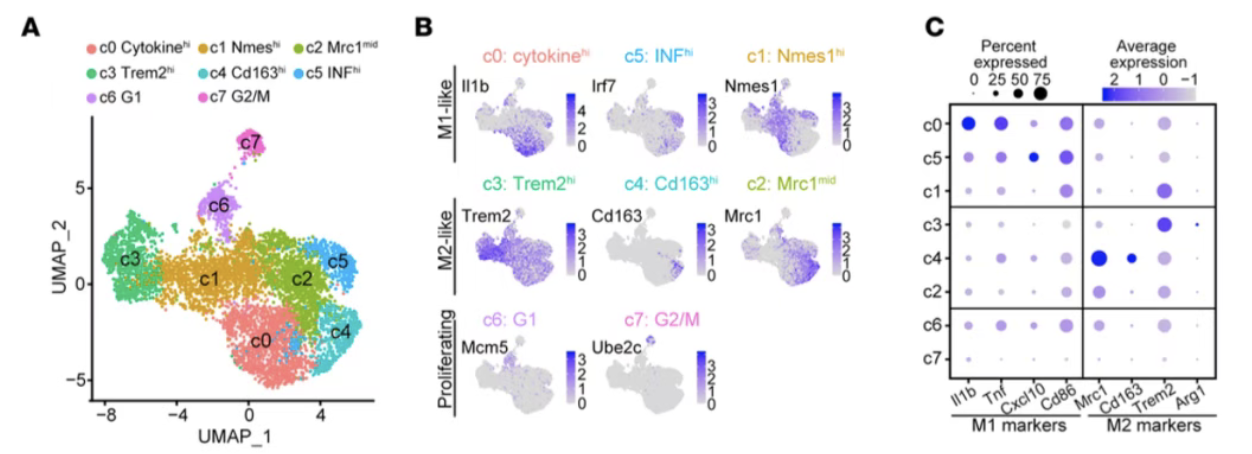
\includegraphics[width=\textwidth,keepaspectratio]{utils/imgs/sample1.png}
    \caption{sample figure}
    \label{fig:sample_figure1}
\end{figure}
		\newpage
		\modified{\lipsum[3]} \added{The results are shown in Table~\ref{tab:table1}. }
		% Requires: \usepackage{booktabs}
\begin{table}[H]
    \centering
    \begin{addedenv}
    \caption{Example table (header + two data rows).}
    \label{tab:table1}
    \begin{tabular}{lcccc}
    \toprule
    Item & Feature 1 & Feature 2 & Feature 3 & Feature 4 \\
    \midrule
    Sample 1 & 12.4 & 0.86 & 45 & 7.9 \\
    Sample 2 & 10.1 & 0.73 & 39 & 8.4 \\
    \cellcolor[HTML]{F9D7EF}Ours & \cellcolor[HTML]{F9D7EF}11.2 & \cellcolor[HTML]{F9D7EF}0.78 & \cellcolor[HTML]{F9D7EF}42 & \cellcolor[HTML]{F9D7EF}8.1 \\
    \bottomrule
    \end{tabular}
    \end{addedenv}
\end{table}
    
		
	\end{changes}
	
\end{revresponse}

\begin{revcomment}
The paper is not clear about the application of the proposed methods.
\end{revcomment}
\begin{revresponse}[]
    Thank you for your constructive suggestions. \lipsum[6] \cite{tomsett2020rapid,liu2019large,qi2023text} The figure is shown in Figure~\ref{fig:sample_figure2}.
    \begin{figure}[H]
    \centering
    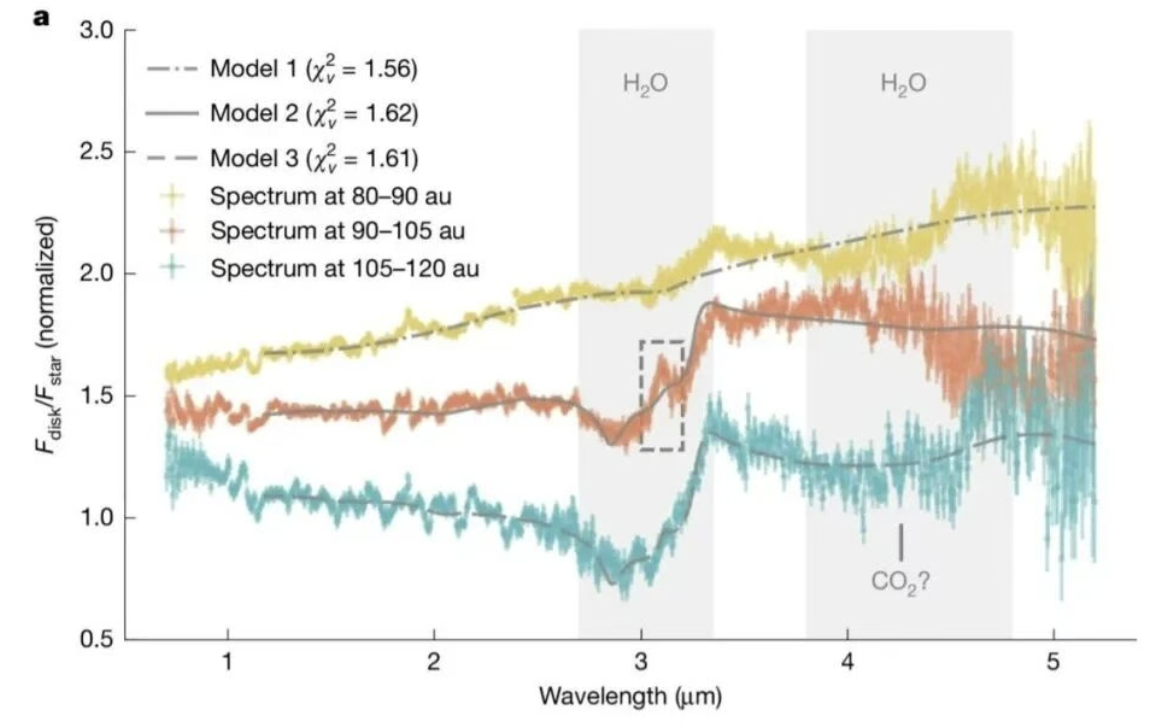
\includegraphics[width=0.8\textwidth,keepaspectratio]{utils/imgs/sample2.png}
    \caption{sample figure 2}
    \label{fig:sample_figure2}
\end{figure}

    \lipsum[7] \cite{zhang2023deep,fu2022long} The algorithm is shown in Algorithm~\ref{algo:dsu}.
    \begin{algorithm}[H]
    \caption{Disjoint Set Union (Union--Find) with Path Compression and Union by Rank (Generated by AI)}
    \label{algo:dsu}
    \begin{algorithmic}[1]
      \Require A finite set $U = \{1,\dots,n\}$; a list of union operations
      \Ensure Ability to query whether two elements are in the same set
      \Statex
      \Function{MakeSet}{$n$}
        \For{$i \gets 1$ \textbf{to} $n$}
          \State parent[$i$] $\gets i$
          \State rank[$i$] $\gets 0$
        \EndFor
      \EndFunction
      \Statex
      \Function{Find}{$x$}
        \If{parent[$x$] $\ne x$}
          \State parent[$x$] $\gets$ \Call{Find}{parent[$x$]} \Comment{Path compression}
        \EndIf
        \State \Return parent[$x$]
      \EndFunction
      \Statex
      \Function{Union}{$x, y$}
        \State $rx \gets$ \Call{Find}{$x$}; \quad $ry \gets$ \Call{Find}{$y$}
        \If{$rx = ry$} \State \Return \EndIf
        \If{rank[$rx$] $<$ rank[$ry$]}
          \State parent[$rx$] $\gets ry$
        \ElsIf{rank[$rx$] $>$ rank[$ry$]}
          \State parent[$ry$] $\gets rx$
        \Else
          \State parent[$ry$] $\gets rx$; \quad rank[$rx$] $\gets$ rank[$rx$] $+ 1$
        \EndIf
      \EndFunction
      \Statex
      \Function{SameSet}{$a, b$}
        \State \Return \Call{Find}{$a$} $=$ \Call{Find}{$b$}
      \EndFunction
    \end{algorithmic}
  \end{algorithm}
  

\end{revresponse}

\clearpage
\printbibliography[heading=bibintoc, heading=bibliography, title={References}, section=\therefsection]

\end{document}